\subsection{Classification}
Our best training on the aforementioned dataset was made with 300 000 iterations over minibatches of size 32, with a learning rate decresaing 10 times throughout training. The full training took 5 days to finish on a Tesla K20C machine, and attained 70\% accuracy on network predictions, on a top-1 classification basis. Such results are satisfactory considering the resemblance of natural scene images. It should be noted that classification was not the main goal, but a good classification will intuitively lead to better class representations.

We can thus extract the trained filters responses to see images as processed by the network. The conv1 layer will mostly learn edges, namely the skyline and the waterline. Conv2 detects foliage, and convolutional layers 3 through 5 contain low-level features that are harder to interpret properly. We tested prototype generation on all convolutional layers, as well as the last pooling layer pool5.

We generated prototypes (some results still pending, will modify when tested) for all classes, and tested whether an image can be recognized only using its class prototypes. Testing over a thousand random images and measuring using a cosine distance shows that all layers perform well for classification. [WILL INCLUDE STATS LIKE MEDIAN DISTANCE]

\begin{figure}[htb]
\centering
\begin{tabular}{cc}
    \bmvaHangBox{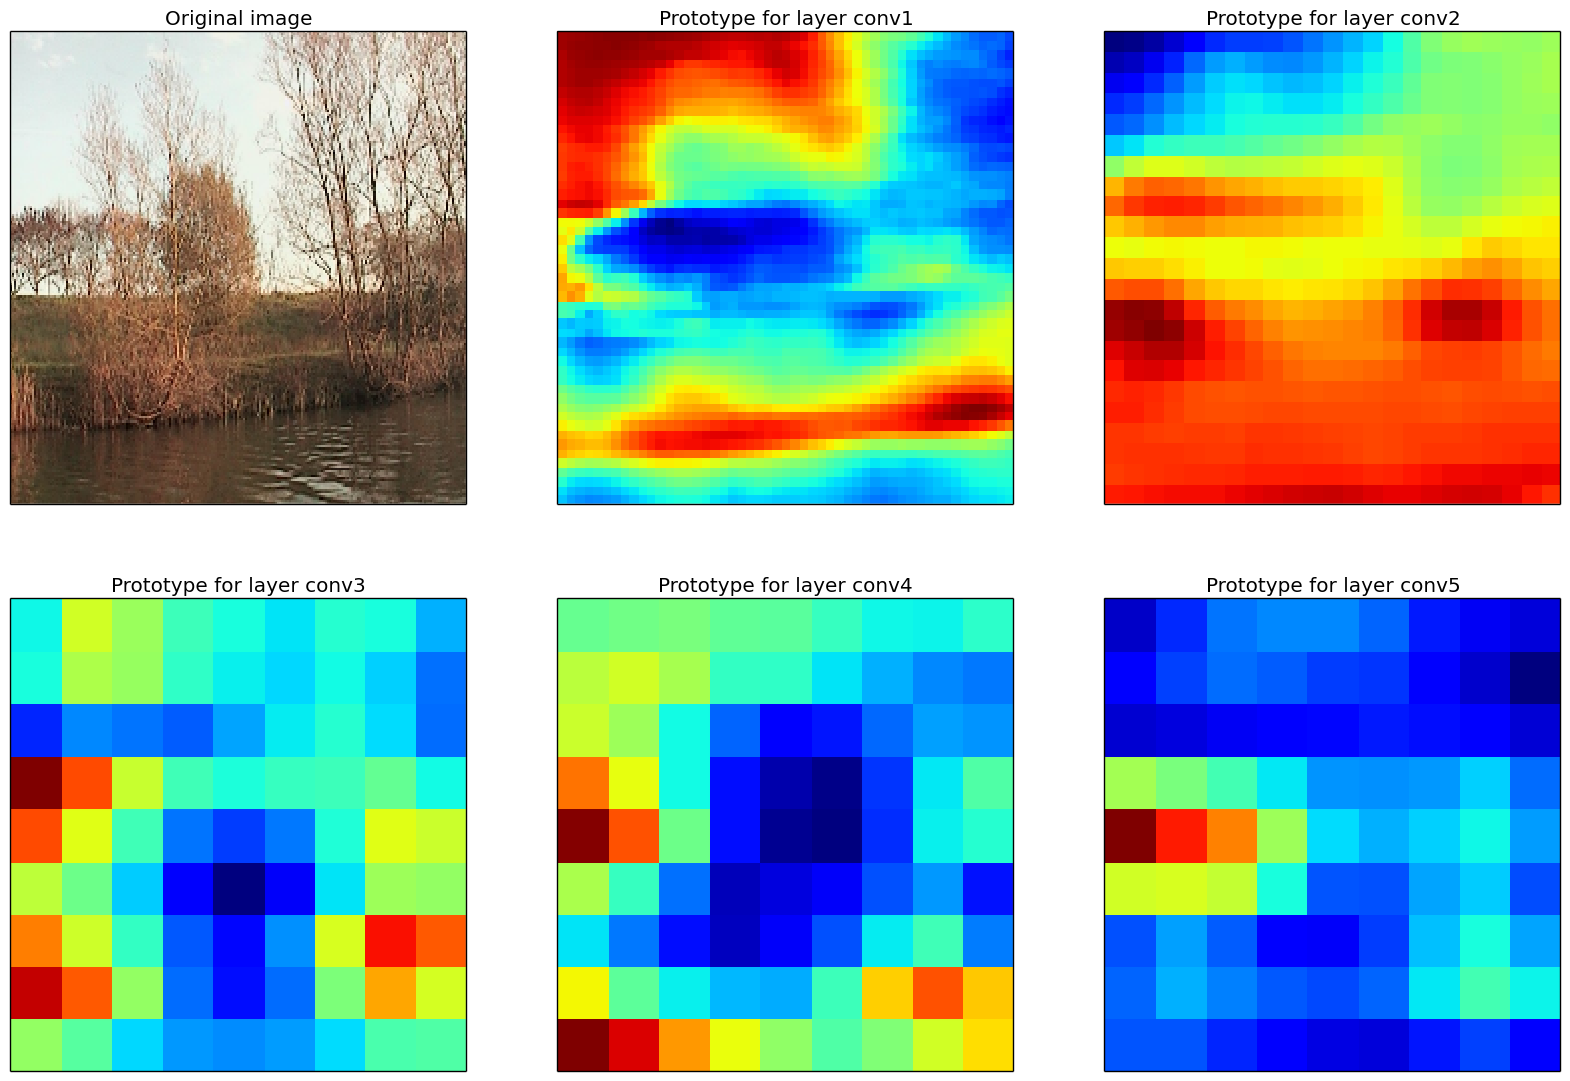
\includegraphics[width=0.66\linewidth]{images/classification/prototypes/avmaskplot7}}\\
\end{tabular}
\caption{Example of prototypes for a given image}
\label{prototypes}
\end{figure}

We also trained the same network on half the classes, to test for generalization capabilities. We observed the same results as before on known classes, and found that pool5 is just as good on unknown classes. The pool5 layer is thus a great choice of seasonal-invariant representation, being both compact and able to generalize.

\begin{figure}[htb]
\centering
\begin{tabular}{ccc}
    a) All classes, full train & b) Unseen classes, half train & c) Seen classes, half train \\
    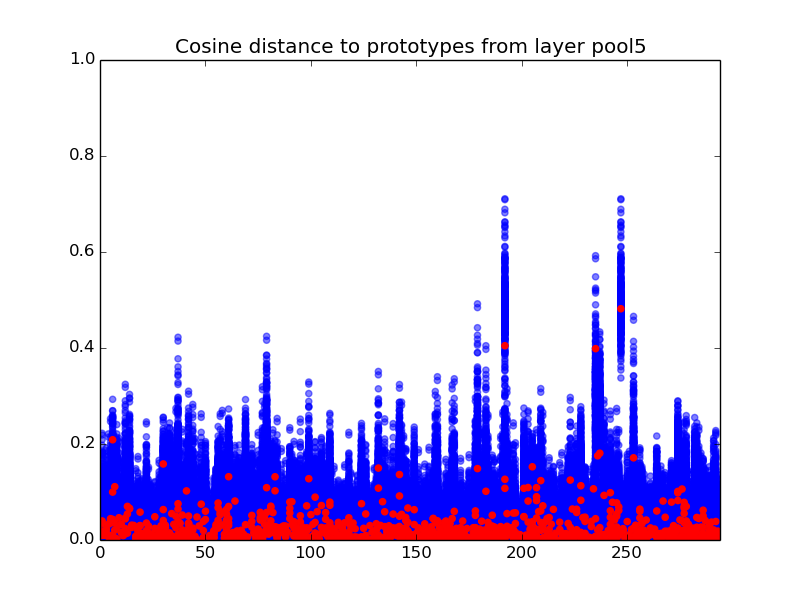
\includegraphics[width=0.33\linewidth]{images/classification/distances/all_classes_full_train/cos_distances_pool5}&
    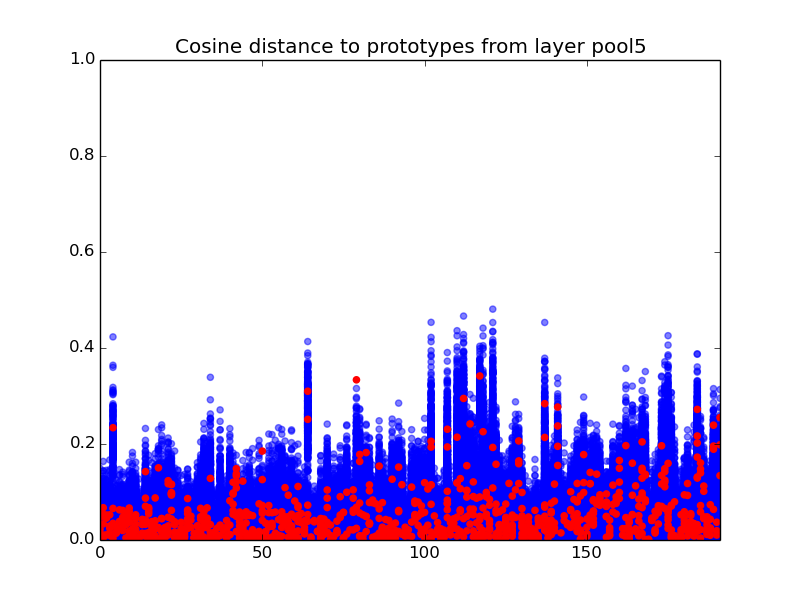
\includegraphics[width=0.33\linewidth]{images/classification/distances/down_distances_up_train/cos_distances_pool5}&
    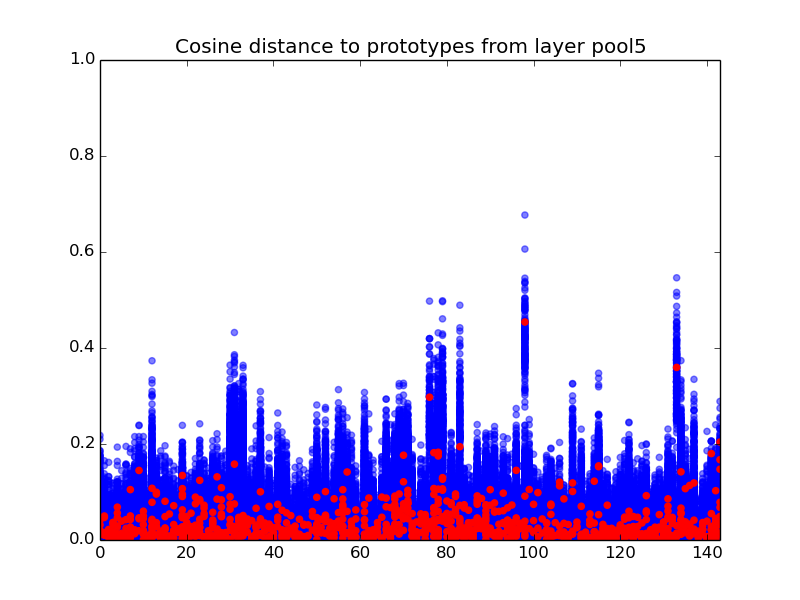
\includegraphics[width=0.33\linewidth]{images/classification/distances/up_distances_up_train/cos_distances_pool5}\\
\end{tabular}
\caption{Red dots represent the distance from a random class image to its class prototype, blue dots are distances to other class prototypes. The pool5 prototypes yield the best results as representations. }
\label{allclft}
\label{dwnclupt}
\label{upclupt}
\end{figure}